\chapter{A Formal Explainer for Just-In-Time Defect Predictions}\label{chap:jit}

This chapter is based on:
\begin{itemize}
	\item Jinqiang Yu, Michael Fu, Alexey Ignatiev, Chakkrit Tantithamthavorn, and Peter J. Stuckey. A
Formal Explainer for Just-In-Time Defect Predictions. \emph{ACM Transactions on Software Engineering
	and Methodology,} 2024. (\textbf{Accepted.})
\end{itemize}

Software companies often rapidly release software products at a rapid pace in short-term development
cycles.
%
The rapid pace of software release presents significant challenges
because of the exponential increase of highly complex source code, particularly for 
under-resourced software quality assurance~(SQA) teams.
%
Due to the time-consuming and costly nature of various SQA activities, 
e.g., code review, developers are unable to thoroughly guarantee the highest quality for 
all newly developed code commits or pull requests given limited time and resources.
%
Just-in-Time (JIT) defect prediction~\cite{kim2007predicting,Kamei2013,pornprasit2021jitline,lin2021impact} is 
proposed to predict whether a commit will introduce software defects in the future. 
%
This allows teams to allocate their finite SQA resources to the most critical 
commits or pull requests. 
%
However, JIT defect prediction largely remains a black-box approach, 
offering predictions that lack explainability and actionable insights for practitioners.
%
Previous research has applied a range of model-agnostic techniques to explain the predictions made
by JIT models.
%
Unfortunately, explanations produced by these methods are still not formally sound, robust, and
actionable.
%
Motivated by the limitation of model-agnostic approaches, this chapter introduces FoX, 
a Formal eXplainer for JIT defect prediction.
%
With the use of formal reasoning about the functionality of JIT defect prediction models,
FoX can offer explanations that are not only provably correct but also guaranteed to be 
minimal.
%
Experimental results demonstrate that FoX can effectively produce explanations that are provably correct, correct,
and actionable. 
%
In contrast, explanations generated by model-agnostic methods do not hold this
%
The survey conducted among 54 software practitioners offers valuable insights 
into the usefulness and trustworthiness of FoX.
%
74\% of respondents found it to be trustworthy,
and 86\% agreed with the usefulness of FoX.
%
Hence, this chapter serves as a significant advancement towards providing trustable explanations for
JIT models, enabling domain experts and practitioners to gain a clearer understanding of
why a commit is predicted as defective and how to mitigate the risk.

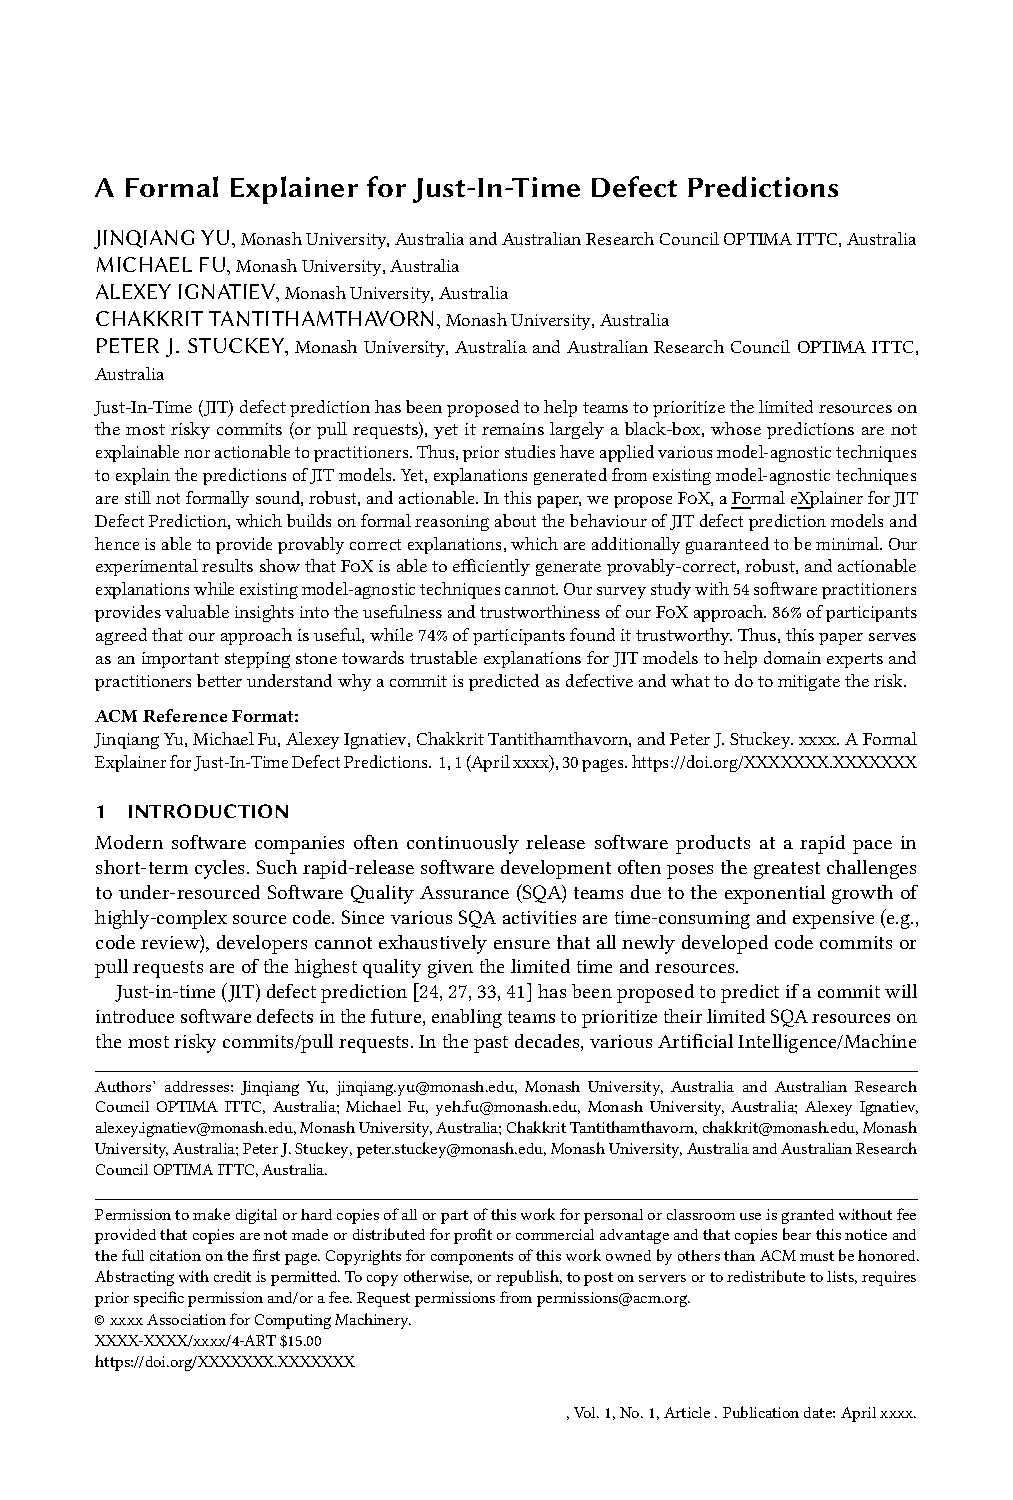
\includepdf[pages=-, offset=75 -75]{papers/jit.pdf}
